The correctness of the leaf-level components introduced by CASE
transformations resolves to the question of whether such a component
meets its AGREE contract. This proof obligation is approachable in
various ways: for example, it can be dealt with by inspection, unit
testing, or by formal proof. In CASE, we take a version of the formal
proof route: \emph{synthesis}. In particular, given a sufficiently
detailed formal contract, we generate code from it and generate proofs
showing that the generated code obeys the contract.

The formal languages that filters, gates, and monitors are generated
from include regular expressions, \cite{case-verified-filter},
contiguity types \cite{contiguity-types}, and Lustre. For each of
these languages, we have infrastructure (see Figure
\ref{fig:synthesis} that (a) translates formal specifications to code
and (b) proves the correctness of the translation. The generated code
is CakeML \cite{cakeml}, a verified compiler for a Standard ML
variant.

\begin{figure}[h]
\begin{center}
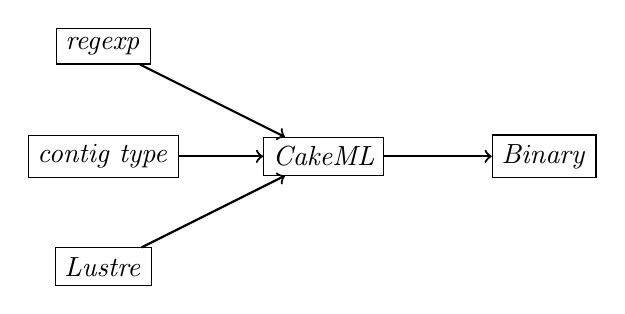
\begin{tikzpicture}[scale = 0.7]
\node (A) at (0,2) [shape=rectangle,draw]{\textit{regexp}};
\node (B) at (0,0) [shape=rectangle,draw]{\textit{contig type}};
\node (C) at (0,-2) [shape=rectangle,draw]{\textit{Lustre}};
\node (D) at (4,0) [shape=rectangle,draw]{\textit{CakeML}};
\node (E) at (8,0) [shape=rectangle,draw]{\textit{Binary}};
\draw [->,thick] (A) to (D);
\draw [->,thick] (B) to (D);
\draw [->,thick] (C) to (D);
\draw [->,thick] (D) to (E);
\end{tikzpicture}
\end{center}
\caption{Synthesis path.\label{fig:synthesis}}
\end{figure}
